    \begin{subfigure}[c]{0.4\textwidth}
    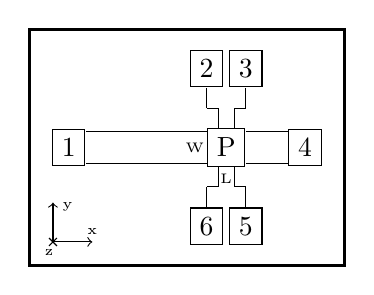
\begin{tikzpicture}
        % Koordinaten
        \draw [<->] (-0.2,-0.7) -- (-0.2,-1.2) -- (0.3,-1.2);
        \draw (-0.15,-1.15) -- (-0.25,-1.25);
        \draw (-0.15,-1.25) -- (-0.25,-1.15);
        \draw (0.3,-1.23) node[anchor=south] {\tiny x};
        \draw (-0.2,-0.75) node[anchor=west] {\tiny y};
        \draw (-0.25,-1.17) node[anchor=north] {\tiny z};
        % Rahmen
        \draw [very thick] (-0.5,-1.5) rectangle (3.5,1.5);
        %Bauelemente
        \draw (0,0) node[rectangle,draw] {1};
        \draw (2,0) node[rectangle,draw] {P};
        \draw (3,0) node[rectangle,draw] {4};
        \draw (1.75, 1) node[rectangle,draw] {2};
        \draw (2.25, 1) node[rectangle,draw] {3};
        \draw (1.75,-1) node[rectangle,draw] {6};
        \draw (2.25,-1) node[rectangle,draw] {5};
        % W, L
        \draw (1.6, 0  ) node {\tiny W};
        \draw (2  ,-0.4) node {\tiny L};
        % Kabel 1
        \draw (0.22,-0.2) -- (1.75,-0.2);
        \draw (0.22,0.2) -- (1.75,0.2);
        % Kabel 4
        \draw (2.25,-0.2) -- (2.78,-0.2);
        \draw (2.25, 0.2) -- (2.78, 0.2);
        % Kabel 2
        \draw (1.75,0.75) -- (1.75,0.5);
        \draw (1.75, 0.5) -- (1.9,0.5);
        \draw (1.9 , 0.5) -- (1.9,0.25);
        % Kabel 3
        \draw (2.25,0.75) -- (2.25,0.5);
        \draw (2.25, 0.5) -- (2.1,0.5);
        \draw (2.1 , 0.5) -- (2.1,0.25);
        % Kabel 6
        \draw (1.75,-0.75) -- (1.75,-0.5);
        \draw (1.75,- 0.5) -- (1.9, -0.5);
        \draw (1.9 ,- 0.5) -- (1.9, -0.25);
        % Kabel 3
        \draw (2.25,-0.75) -- (2.25,-0.5);
        \draw (2.25,- 0.5) -- (2.1, -0.5);
        \draw (2.1 ,- 0.5) -- (2.1, -0.25);
    \end{tikzpicture}
    \end{subfigure}
